\documentclass{standalone} 
         \usepackage{graphicx} 
 \usepackage[hang,small,bf]{caption}    % fancy captions
 \usepackage{tikz}	

% TikZ libraries 
\usetikzlibrary{shapes,snakes} 
\usetikzlibrary{backgrounds,fit,decorations.pathreplacing} 
 \usetikzlibrary{shapes,arrows,fit,calc,positioning,automata} 
\newcommand{\ket}[1]{\ensuremath{\left|#1\right\rangle}} % Dirac Kets 
\begin{document} 
    %\begin{figure} 
    %\centerline{ 
        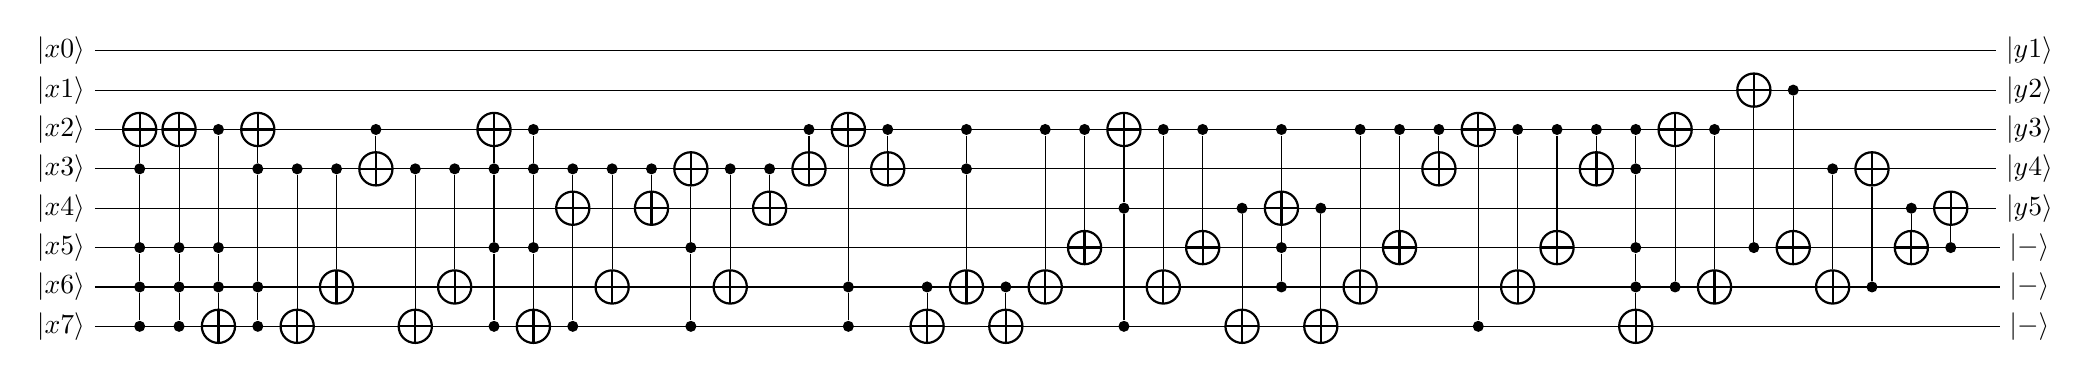
\begin{tikzpicture}[] 
            \tikzset{oplus/.style={path picture={% 
            \draw[black] 
            (path picture bounding box.south) -- (path picture bounding box.north) 
            (path picture bounding box.west) -- (path picture bounding box.east);
            }}}
             \tikzstyle{operator} = [draw,fill=white,minimum size=1.5em] 
             \tikzstyle{phase} = [fill,shape=circle,minimum size=4pt,inner sep=0pt]
             \tikzstyle{surround} = [fill=blue!10,thick,draw=black,rounded corners=2mm]
             \tikzstyle{swap} = [draw,fill,shape=cross out,minimum size=5pt,inner sep=0pt]
             \tikzstyle{cnot} = [oplus,draw,thick,circle,minimum size = 12pt]		% Qubit
		\node at (0,-0.0)(q0_0) {\ket{x0}};
		\node at (0,-0.5)(q0_1) {\ket{x1}};
		\node at (0,-1.0)(q0_2) {\ket{x2}};
		\node at (0,-1.5)(q0_3) {\ket{x3}};
		\node at (0,-2.0)(q0_4) {\ket{x4}};
		\node at (0,-2.5)(q0_5) {\ket{x5}};
		\node at (0,-3.0)(q0_6) {\ket{x6}};
		\node at (0,-3.5)(q0_7) {\ket{x7}};
		% Gate 1
		\node[phase] (q1_3) at (1.0,-1.5) {} edge [-] (q0_3);
		\node[phase] (q1_5) at (1.0,-2.5) {} edge [-] (q0_5);
		\node[phase] (q1_6) at (1.0,-3.0) {} edge [-] (q0_6);
		\node[phase] (q1_7) at (1.0,-3.5) {} edge [-] (q0_7);
		\node[cnot] (q1_2) at (1.0,-1.0) {} edge [-] (q0_2);
		\draw[-] (q1_2)  -- (q1_3);
		\draw[-] (q1_3)  -- (q1_5);
		\draw[-] (q1_5)  -- (q1_6);
		\draw[-] (q1_6)  -- (q1_7);
		% Gate 2
		\node[phase] (q2_5) at (1.5,-2.5) {} edge [-] (q1_5);
		\node[phase] (q2_6) at (1.5,-3.0) {} edge [-] (q1_6);
		\node[phase] (q2_7) at (1.5,-3.5) {} edge [-] (q1_7);
		\node[cnot] (q2_2) at (1.5,-1.0) {} edge [-] (q1_2);
		\draw[-] (q2_2)  -- (q2_5);
		\draw[-] (q2_5)  -- (q2_6);
		\draw[-] (q2_6)  -- (q2_7);
		% Gate 3
		\node[phase] (q3_2) at (2.0,-1.0) {} edge [-] (q2_2);
		\node[phase] (q3_5) at (2.0,-2.5) {} edge [-] (q2_5);
		\node[phase] (q3_6) at (2.0,-3.0) {} edge [-] (q2_6);
		\node[cnot] (q3_7) at (2.0,-3.5) {} edge [-] (q2_7);
		\draw[-] (q3_2)  -- (q3_5);
		\draw[-] (q3_5)  -- (q3_6);
		\draw[-] (q3_6)  -- (q3_7);
		% Gate 4
		\node[phase] (q4_3) at (2.5,-1.5) {} edge [-] (q1_3);
		\node[phase] (q4_6) at (2.5,-3.0) {} edge [-] (q3_6);
		\node[phase] (q4_7) at (2.5,-3.5) {} edge [-] (q3_7);
		\node[cnot] (q4_2) at (2.5,-1.0) {} edge [-] (q3_2);
		\draw[-] (q4_2)  -- (q4_3);
		\draw[-] (q4_3)  -- (q4_6);
		\draw[-] (q4_6)  -- (q4_7);
		% Gate 5
		\node[phase] (q5_3) at (3.0,-1.5) {} edge [-] (q4_3);
		\node[cnot] (q5_7) at (3.0,-3.5) {} edge [-] (q4_7);
		\draw[-] (q5_3)  -- (q5_7);
		% Gate 6
		\node[phase] (q6_3) at (3.5,-1.5) {} edge [-] (q5_3);
		\node[cnot] (q6_6) at (3.5,-3.0) {} edge [-] (q4_6);
		\draw[-] (q6_3)  -- (q6_6);
		% Gate 7
		\node[phase] (q7_2) at (4.0,-1.0) {} edge [-] (q4_2);
		\node[cnot] (q7_3) at (4.0,-1.5) {} edge [-] (q6_3);
		\draw[-] (q7_2)  -- (q7_3);
		% Gate 8
		\node[phase] (q8_3) at (4.5,-1.5) {} edge [-] (q7_3);
		\node[cnot] (q8_7) at (4.5,-3.5) {} edge [-] (q5_7);
		\draw[-] (q8_3)  -- (q8_7);
		% Gate 9
		\node[phase] (q9_3) at (5.0,-1.5) {} edge [-] (q8_3);
		\node[cnot] (q9_6) at (5.0,-3.0) {} edge [-] (q6_6);
		\draw[-] (q9_3)  -- (q9_6);
		% Gate 10
		\node[phase] (q10_3) at (5.5,-1.5) {} edge [-] (q9_3);
		\node[phase] (q10_5) at (5.5,-2.5) {} edge [-] (q3_5);
		\node[phase] (q10_7) at (5.5,-3.5) {} edge [-] (q8_7);
		\node[cnot] (q10_2) at (5.5,-1.0) {} edge [-] (q7_2);
		\draw[-] (q10_2)  -- (q10_3);
		\draw[-] (q10_3)  -- (q10_5);
		\draw[-] (q10_5)  -- (q10_7);
		% Gate 11
		\node[phase] (q11_2) at (6.0,-1.0) {} edge [-] (q10_2);
		\node[phase] (q11_3) at (6.0,-1.5) {} edge [-] (q10_3);
		\node[phase] (q11_5) at (6.0,-2.5) {} edge [-] (q10_5);
		\node[cnot] (q11_7) at (6.0,-3.5) {} edge [-] (q10_7);
		\draw[-] (q11_2)  -- (q11_3);
		\draw[-] (q11_3)  -- (q11_5);
		\draw[-] (q11_5)  -- (q11_7);
		% Gate 12
		\node[phase] (q12_3) at (6.5,-1.5) {} edge [-] (q11_3);
		\node[phase] (q12_7) at (6.5,-3.5) {} edge [-] (q11_7);
		\node[cnot] (q12_4) at (6.5,-2.0) {} edge [-] (q0_4);
		\draw[-] (q12_3)  -- (q12_4);
		\draw[-] (q12_4)  -- (q12_7);
		% Gate 13
		\node[phase] (q13_3) at (7.0,-1.5) {} edge [-] (q12_3);
		\node[cnot] (q13_6) at (7.0,-3.0) {} edge [-] (q9_6);
		\draw[-] (q13_3)  -- (q13_6);
		% Gate 14
		\node[phase] (q14_3) at (7.5,-1.5) {} edge [-] (q13_3);
		\node[cnot] (q14_4) at (7.5,-2.0) {} edge [-] (q12_4);
		\draw[-] (q14_3)  -- (q14_4);
		% Gate 15
		\node[phase] (q15_5) at (8.0,-2.5) {} edge [-] (q11_5);
		\node[phase] (q15_7) at (8.0,-3.5) {} edge [-] (q12_7);
		\node[cnot] (q15_3) at (8.0,-1.5) {} edge [-] (q14_3);
		\draw[-] (q15_3)  -- (q15_5);
		\draw[-] (q15_5)  -- (q15_7);
		% Gate 16
		\node[phase] (q16_3) at (8.5,-1.5) {} edge [-] (q15_3);
		\node[cnot] (q16_6) at (8.5,-3.0) {} edge [-] (q13_6);
		\draw[-] (q16_3)  -- (q16_6);
		% Gate 17
		\node[phase] (q17_3) at (9.0,-1.5) {} edge [-] (q16_3);
		\node[cnot] (q17_4) at (9.0,-2.0) {} edge [-] (q14_4);
		\draw[-] (q17_3)  -- (q17_4);
		% Gate 18
		\node[phase] (q18_2) at (9.5,-1.0) {} edge [-] (q11_2);
		\node[cnot] (q18_3) at (9.5,-1.5) {} edge [-] (q17_3);
		\draw[-] (q18_2)  -- (q18_3);
		% Gate 19
		\node[phase] (q19_6) at (10.0,-3.0) {} edge [-] (q16_6);
		\node[phase] (q19_7) at (10.0,-3.5) {} edge [-] (q15_7);
		\node[cnot] (q19_2) at (10.0,-1.0) {} edge [-] (q18_2);
		\draw[-] (q19_2)  -- (q19_6);
		\draw[-] (q19_6)  -- (q19_7);
		% Gate 20
		\node[phase] (q20_2) at (10.5,-1.0) {} edge [-] (q19_2);
		\node[cnot] (q20_3) at (10.5,-1.5) {} edge [-] (q18_3);
		\draw[-] (q20_2)  -- (q20_3);
		% Gate 21
		\node[phase] (q21_6) at (11.0,-3.0) {} edge [-] (q19_6);
		\node[cnot] (q21_7) at (11.0,-3.5) {} edge [-] (q19_7);
		\draw[-] (q21_6)  -- (q21_7);
		% Gate 22
		\node[phase] (q22_2) at (11.5,-1.0) {} edge [-] (q20_2);
		\node[phase] (q22_3) at (11.5,-1.5) {} edge [-] (q20_3);
		\node[cnot] (q22_6) at (11.5,-3.0) {} edge [-] (q21_6);
		\draw[-] (q22_2)  -- (q22_3);
		\draw[-] (q22_3)  -- (q22_6);
		% Gate 23
		\node[phase] (q23_6) at (12.0,-3.0) {} edge [-] (q22_6);
		\node[cnot] (q23_7) at (12.0,-3.5) {} edge [-] (q21_7);
		\draw[-] (q23_6)  -- (q23_7);
		% Gate 24
		\node[phase] (q24_2) at (12.5,-1.0) {} edge [-] (q22_2);
		\node[cnot] (q24_6) at (12.5,-3.0) {} edge [-] (q23_6);
		\draw[-] (q24_2)  -- (q24_6);
		% Gate 25
		\node[phase] (q25_2) at (13.0,-1.0) {} edge [-] (q24_2);
		\node[cnot] (q25_5) at (13.0,-2.5) {} edge [-] (q15_5);
		\draw[-] (q25_2)  -- (q25_5);
		% Gate 26
		\node[phase] (q26_4) at (13.5,-2.0) {} edge [-] (q17_4);
		\node[phase] (q26_7) at (13.5,-3.5) {} edge [-] (q23_7);
		\node[cnot] (q26_2) at (13.5,-1.0) {} edge [-] (q25_2);
		\draw[-] (q26_2)  -- (q26_4);
		\draw[-] (q26_4)  -- (q26_7);
		% Gate 27
		\node[phase] (q27_2) at (14.0,-1.0) {} edge [-] (q26_2);
		\node[cnot] (q27_6) at (14.0,-3.0) {} edge [-] (q24_6);
		\draw[-] (q27_2)  -- (q27_6);
		% Gate 28
		\node[phase] (q28_2) at (14.5,-1.0) {} edge [-] (q27_2);
		\node[cnot] (q28_5) at (14.5,-2.5) {} edge [-] (q25_5);
		\draw[-] (q28_2)  -- (q28_5);
		% Gate 29
		\node[phase] (q29_4) at (15.0,-2.0) {} edge [-] (q26_4);
		\node[cnot] (q29_7) at (15.0,-3.5) {} edge [-] (q26_7);
		\draw[-] (q29_4)  -- (q29_7);
		% Gate 30
		\node[phase] (q30_2) at (15.5,-1.0) {} edge [-] (q28_2);
		\node[phase] (q30_5) at (15.5,-2.5) {} edge [-] (q28_5);
		\node[phase] (q30_6) at (15.5,-3.0) {} edge [-] (q27_6);
		\node[cnot] (q30_4) at (15.5,-2.0) {} edge [-] (q29_4);
		\draw[-] (q30_2)  -- (q30_4);
		\draw[-] (q30_4)  -- (q30_5);
		\draw[-] (q30_5)  -- (q30_6);
		% Gate 31
		\node[phase] (q31_4) at (16.0,-2.0) {} edge [-] (q30_4);
		\node[cnot] (q31_7) at (16.0,-3.5) {} edge [-] (q29_7);
		\draw[-] (q31_4)  -- (q31_7);
		% Gate 32
		\node[phase] (q32_2) at (16.5,-1.0) {} edge [-] (q30_2);
		\node[cnot] (q32_6) at (16.5,-3.0) {} edge [-] (q30_6);
		\draw[-] (q32_2)  -- (q32_6);
		% Gate 33
		\node[phase] (q33_2) at (17.0,-1.0) {} edge [-] (q32_2);
		\node[cnot] (q33_5) at (17.0,-2.5) {} edge [-] (q30_5);
		\draw[-] (q33_2)  -- (q33_5);
		% Gate 34
		\node[phase] (q34_2) at (17.5,-1.0) {} edge [-] (q33_2);
		\node[cnot] (q34_3) at (17.5,-1.5) {} edge [-] (q22_3);
		\draw[-] (q34_2)  -- (q34_3);
		% Gate 35
		\node[phase] (q35_7) at (18.0,-3.5) {} edge [-] (q31_7);
		\node[cnot] (q35_2) at (18.0,-1.0) {} edge [-] (q34_2);
		\draw[-] (q35_2)  -- (q35_7);
		% Gate 36
		\node[phase] (q36_2) at (18.5,-1.0) {} edge [-] (q35_2);
		\node[cnot] (q36_6) at (18.5,-3.0) {} edge [-] (q32_6);
		\draw[-] (q36_2)  -- (q36_6);
		% Gate 37
		\node[phase] (q37_2) at (19.0,-1.0) {} edge [-] (q36_2);
		\node[cnot] (q37_5) at (19.0,-2.5) {} edge [-] (q33_5);
		\draw[-] (q37_2)  -- (q37_5);
		% Gate 38
		\node[phase] (q38_2) at (19.5,-1.0) {} edge [-] (q37_2);
		\node[cnot] (q38_3) at (19.5,-1.5) {} edge [-] (q34_3);
		\draw[-] (q38_2)  -- (q38_3);
		% Gate 39
		\node[phase] (q39_2) at (20.0,-1.0) {} edge [-] (q38_2);
		\node[phase] (q39_3) at (20.0,-1.5) {} edge [-] (q38_3);
		\node[phase] (q39_5) at (20.0,-2.5) {} edge [-] (q37_5);
		\node[phase] (q39_6) at (20.0,-3.0) {} edge [-] (q36_6);
		\node[cnot] (q39_7) at (20.0,-3.5) {} edge [-] (q35_7);
		\draw[-] (q39_2)  -- (q39_3);
		\draw[-] (q39_3)  -- (q39_5);
		\draw[-] (q39_5)  -- (q39_6);
		\draw[-] (q39_6)  -- (q39_7);
		% Gate 40
		\node[phase] (q40_6) at (20.5,-3.0) {} edge [-] (q39_6);
		\node[cnot] (q40_2) at (20.5,-1.0) {} edge [-] (q39_2);
		\draw[-] (q40_2)  -- (q40_6);
		% Gate 41
		\node[phase] (q41_2) at (21.0,-1.0) {} edge [-] (q40_2);
		\node[cnot] (q41_6) at (21.0,-3.0) {} edge [-] (q40_6);
		\draw[-] (q41_2)  -- (q41_6);
		% Gate 42
		\node[phase] (q42_5) at (21.5,-2.5) {} edge [-] (q39_5);
		\node[cnot] (q42_1) at (21.5,-0.5) {} edge [-] (q0_1);
		\draw[-] (q42_1)  -- (q42_5);
		% Gate 43
		\node[phase] (q43_1) at (22.0,-0.5) {} edge [-] (q42_1);
		\node[cnot] (q43_5) at (22.0,-2.5) {} edge [-] (q42_5);
		\draw[-] (q43_1)  -- (q43_5);
		% Gate 44
		\node[phase] (q44_3) at (22.5,-1.5) {} edge [-] (q39_3);
		\node[cnot] (q44_6) at (22.5,-3.0) {} edge [-] (q41_6);
		\draw[-] (q44_3)  -- (q44_6);
		% Gate 45
		\node[phase] (q45_6) at (23.0,-3.0) {} edge [-] (q44_6);
		\node[cnot] (q45_3) at (23.0,-1.5) {} edge [-] (q44_3);
		\draw[-] (q45_3)  -- (q45_6);
		% Gate 46
		\node[phase] (q46_4) at (23.5,-2.0) {} edge [-] (q31_4);
		\node[cnot] (q46_5) at (23.5,-2.5) {} edge [-] (q43_5);
		\draw[-] (q46_4)  -- (q46_5);
		% Gate 47
		\node[phase] (q47_5) at (24.0,-2.5) {} edge [-] (q46_5);
		\node[cnot] (q47_4) at (24.0,-2.0) {} edge [-] (q46_4);
		\draw[-] (q47_4)  -- (q47_5);
		% Output
		\node at (25.0,-0.0)(q48_0) {\ket{y1}};
		\draw[-] (q0_0)  -- (q48_0);
		\node at (25.0,-0.5)(q48_1) {\ket{y2}};
		\draw[-] (q0_1)  -- (q48_1);
		\node at (25.0,-1.0)(q48_2) {\ket{y3}};
		\draw[-] (q0_2)  -- (q48_2);
		\node at (25.0,-1.5)(q48_3) {\ket{y4}};
		\draw[-] (q0_3)  -- (q48_3);
		\node at (25.0,-2.0)(q48_4) {\ket{y5}};
		\draw[-] (q0_4)  -- (q48_4);
		\node at (25.0,-2.5)(q48_5) {\ket{-}};
		\draw[-] (q0_5)  -- (q48_5);
		\node at (25.0,-3.0)(q48_6) {\ket{-}};
		\draw[-] (q0_6)  -- (q48_6);
		\node at (25.0,-3.5)(q48_7) {\ket{-}};
		\draw[-] (q0_7)  -- (q48_7);
		\end{tikzpicture} 
   %}
%\end{figure}
\end{document}
